\documentclass[tikz,border=4pt]{standalone}
\usepackage[T1]{fontenc}
\usepackage{lmodern}
\usetikzlibrary{arrows.meta,positioning,fit,backgrounds,calc}
\begin{document}
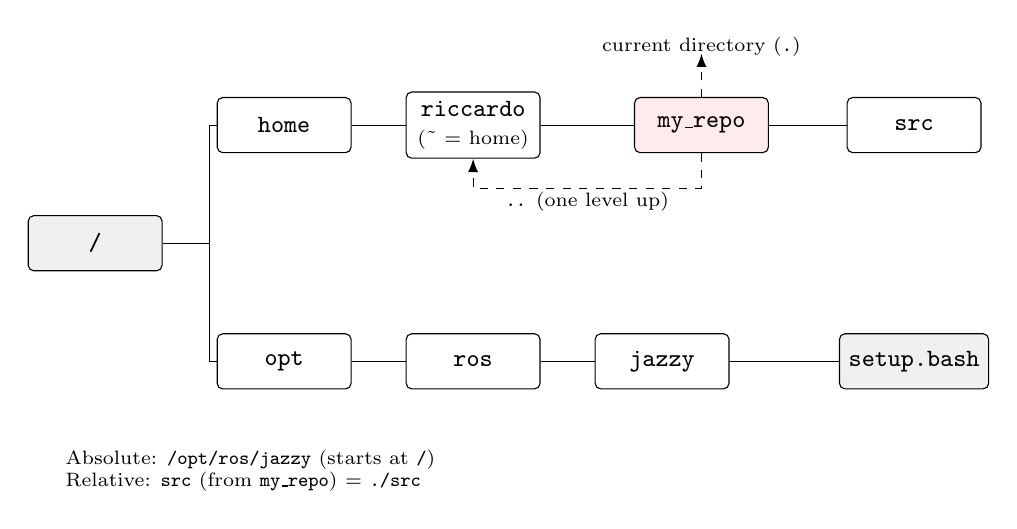
\begin{tikzpicture}[
  blk/.style={draw,rounded corners=2pt,minimum height=7mm,minimum width=17mm,align=center,font=\small,fill=white},
  ros/.style={blk,fill=red!8},
  ext/.style={blk,fill=gray!12},
  lab/.style={font=\scriptsize,fill=white,inner sep=1pt,align=center},
  >={Latex}]
\node[ext] (root) at (0,-1.5) {\texttt{/}};
\node[blk] (home) at (2.4,0) {\texttt{home}};
\node[blk] (usr) at (4.8,0) {\texttt{riccardo}\\[-1pt]\scriptsize (\textasciitilde{} = home)};
\node[ros] (repo) at (7.7,0) {\texttt{my\_repo}};
\node[blk] (src) at (10.4,0) {\texttt{src}};
\node[blk] (opt) at (2.4,-3) {\texttt{opt}};
\node[blk] (rosd) at (4.8,-3) {\texttt{ros}};
\node[blk] (jaz) at (7.2,-3) {\texttt{jazzy}};
\node[ext] (setup) at (10.4,-3) {\texttt{setup.bash}};
\draw (root.east) -- ++(0.6,0) |- (home.west);
\draw (root.east) -- ++(0.6,0) |- (opt.west);
\draw (home) -- (usr);
\draw (usr) -- (repo);
\draw (repo) -- (src);
\draw (opt) -- (rosd);
\draw (rosd) -- (jaz);
\draw (jaz) -- (setup);
\node[font=\scriptsize,anchor=south] at (repo.north |- 0,0.75) {current directory (\texttt{.})};
\draw[->,dashed] (repo.north) -- ++(0,0.55);
\draw[->,dashed] (repo.south) -- ++(0,-0.45) -| node[lab,pos=0.25,below]{\texttt{..} (one level up)} (usr.south);
\node[font=\scriptsize,align=left,anchor=north west] at (-0.5,-4.0)
  {Absolute: \texttt{/opt/ros/jazzy} (starts at \texttt{/})\\
   Relative: \texttt{src} (from \texttt{my\_repo}) = \texttt{./src}};
\end{tikzpicture}
\end{document}
